\documentclass[ngerman,hyperref={pdfpagelabels=false}]{beamer}

% -----------------------------------------------------------------------------

\graphicspath{{images/}}

% -----------------------------------------------------------------------------

\usetheme{KIT}

\setbeamercovered{transparent}
%\setbeamertemplate{enumerate items}[ball]

\newenvironment<>{KITtestblock}[2][]
{\begin{KITcolblock}<#1>{#2}{KITblack15}{KITblack50}}
{\end{KITcolblock}}

\usepackage[ngerman,english]{babel}
\usepackage[utf8]{inputenc}
\usepackage[TS1,T1]{fontenc}
\usepackage{array}
\usepackage{multicol}
\usepackage[absolute,overlay]{textpos}
\usepackage{beamerKITdefs}

\pdfpageattr {/Group << /S /Transparency /I true /CS /DeviceRGB>>}	%required to prevent color shifting withd transparent images


\title{Algorithmen 1 - Tutorium 9}
\subtitle{Sebastian Schmidt -- \textit{isibboi@gmail.com}}

\author[Sebastian Schmidt]{Sebastian Schmidt}
\institute{Arbeitsgruppe Kryptographie und Sicherheit}

\TitleImage[width=\titleimagewd,height=\titleimageht]{graph-theoryjpg}

\KITinstitute{Arbeitsgruppe Kryptographie und Sicherheit}
\KITfaculty{Fakult\"at f\"ur Informatik}

% -----------------------------------------------------------------------------

\begin{document}
\setlength\textheight{7cm} %required for correct vertical alignment, if [t] is not used as documentclass parameter


% title frame
\begin{frame}
  \maketitle
\end{frame}

\begin{frame}{Graphrepräsentationen}

\Large
\only<1-2>{Kantenfolge}
\only<3-4>{Adjazenzfeld}
\only<5-6>{Adjazenzliste}
\only<7-8>{Adjazenzmatrix}

\normalsize
\vspace{1em}
\only<2,4,6,8>{
Operationen/Features:
\begin{itemize}
\item Kantengewichte
\item Knoteninformationen
\item Navigation
\item Eingehende Kanten
\item Rückwärtskante
\item Kanten iterieren
\item Kanten löschen
\item Kanten einfügen
\item Batched Updates
\end{itemize}}
\end{frame}

\begin{frame}{Adjazenzliste++}
\vspace{-1em}
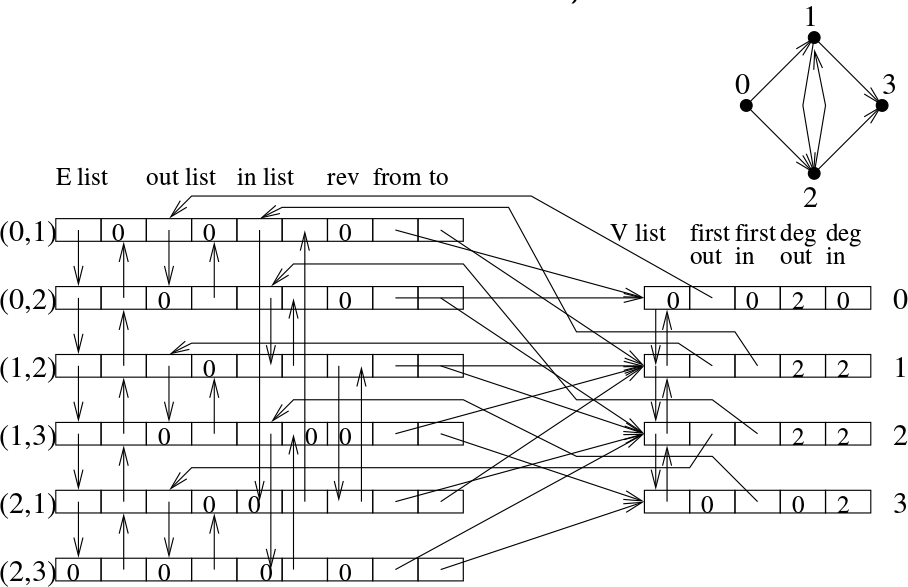
\includegraphics[width=\textwidth]{adjazenzliste++}
\end{frame}

\begin{frame}{Graphtraversierung}
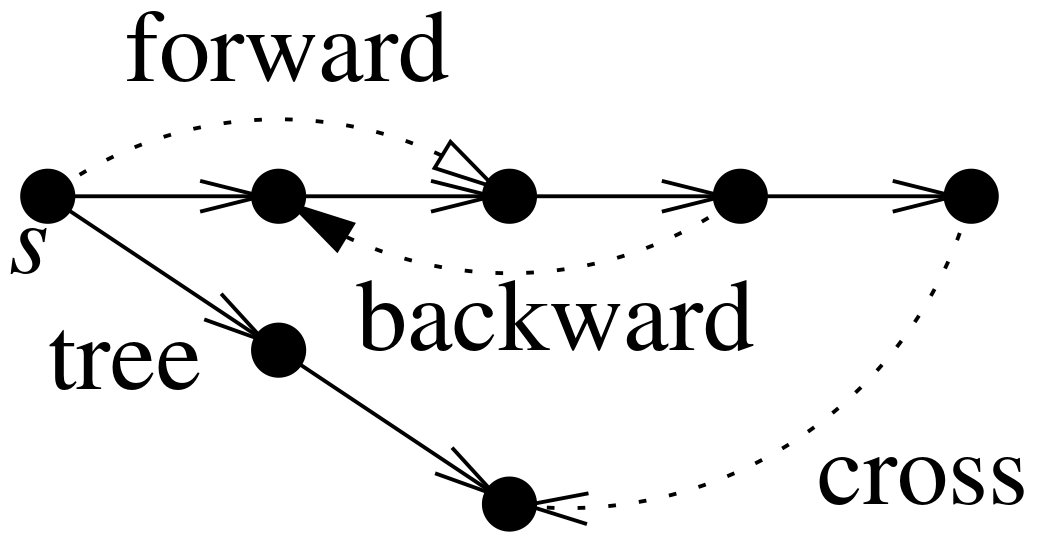
\includegraphics[width=\textwidth]{classes}
\end{frame}

\begin{frame}{Graphtraversierung}
\only<1>{Führe Breitensuche auf einem Beispielgraphen aus.}
\only<2>{Führe Tiefensuche auf einem Beispielgraphen aus.}

\vspace{1em}
Klassifiziere die Kanten als: \emph{tree}, \emph{backward}, \emph{cross}, \emph{forward}
\end{frame}

\begin{frame}
\vspace{-4em}
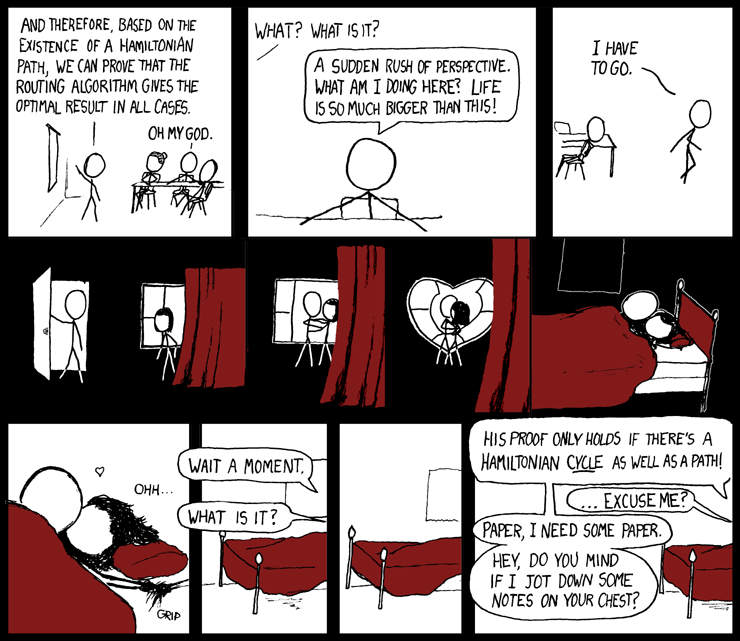
\includegraphics[width=0.85\textwidth]{hamiltonian}
\end{frame}


\end{document}
